\documentclass[a4paper, 12pt]{article}

% Добавляем новые пакеты
\usepackage[english, russian]{babel}    % Пакет для поддержки русского языка
\usepackage[T1, T2A]{fontenc}           % Загружаем пакет с поддержкой кирилицы
\usepackage[utf8]{inputenc}             % Загружаем пакет с поддержкой кодировки файла и символов
\usepackage{ragged2e}                   % Загружаем пакет для выравнивания текста
\usepackage{graphicx}                   % Загружаем пакет для добавления различной графики (pdf, jpg, png)
\usepackage{import}                     % Загружаем пакет для продвинутого импорта, в частности изображений pdf_tex из графического редактора inkscape (\import{<path to file>}{<filename>.pdf_tex})
\usepackage{subcaption}                 % Пакет для поддержки сетки из фигур, например в две колонки или матрицей
\usepackage{float}                      % Пакет для улучшенного размещения изображенией (ниже используется опция H в команде \begin{figure}[H])
\usepackage{geometry}                   % Пакет для управления отступами на странице (см. далее вызываем \geometry)
\usepackage{amsmath}                    % Добавляем крутую поддержку математики, в частности /align
\usepackage{amsfonts}                   % Пкет с мтематическими шрифтами вроде \mathbb и др.
\usepackage{tabu}                       % Пакет с прокаченными таблицами
\usepackage{booktabs}                   % Крутые вертикальные разделители
\usepackage[dvipsnames]{xcolor}         % Рассширенная поддержка цветов
\usepackage[colorlinks]{hyperref}
\usepackage{indentfirst}                % Пакет, чтобы починить красную строку
\usepackage{listings}                   % Поддержка листингов, оформления кода программы
\usepackage{src/vpdtitle}               % Титульный лист (смотри файл vpdtitle.sty)
\usepackage{titletoc}
\usepackage{multirow}
\usepackage{textcomp}
\usepackage{makecell}
\dottedcontents{section}[2.3em]{}{2.3em}{6pt}
\dottedcontents{subsection}[2.3em]{}{2.3em}{6pt}
\dottedcontents{subsubsection}[2.3em]{}{2.3em}{6pt}

% Устанавливает отступы на странице
\geometry{left=2cm, right=2cm, bottom=2cm, top=2cm}

% Настараиваем красивые цвета для ссылок на формулы, фигуры (изображения) и другие элементы.
\hypersetup{
    linkcolor=blue,
    filecolor=magenta,
    urlcolor=cyan
}

% Настраиваем супер красивые листинги с попомщью пакетов listings и xcolor
\definecolor{codegreen}{rgb}{0,0.6,0}
\definecolor{codegray}{rgb}{0.5,0.5,0.5}
\definecolor{codepurple}{rgb}{0.58,0,0.82}
\definecolor{backcolour}{rgb}{0.95,0.95,0.92}

\lstdefinestyle{codestyle}{
    backgroundcolor=\color{backcolour},
    commentstyle=\color{codegreen},
    keywordstyle=\color{magenta},
    numberstyle=\tiny\color{codegray},
    stringstyle=\color{codepurple},
    basicstyle=\ttfamily\footnotesize,
    breakatwhitespace=false,
    breaklines=true,
    captionpos=b,
    keepspaces=true,
    numbers=left,
    numbersep=5pt,
    showspaces=false,
    showstringspaces=false,
    showtabs=false,
    tabsize=2
}

\lstset{style=codestyle}
\lstset{extendedchars=\true}
\lstset{language=Matlab}
\renewcommand{\lstlistingname}{Листинг}

% Кириллица в листингах
\lstset{literate=
    {а}{{\cyra}}1 {б}{{\cyrb}}1 {в}{{\cyrv}}1 {г}{{\cyrg}}1 {д}{{\cyrd}}1 {е}{{\cyre}}1 {ё}{{\cyryo}}1
    {ж}{{\cyrzh}}1 {з}{{\cyrz}}1 {и}{{\cyri}}1 {й}{{\cyrishrt}}1 {к}{{\cyrk}}1 {л}{{\cyrl}}1 {м}{{\cyrm}}1
    {н}{{\cyrn}}1 {о}{{\cyro}}1 {п}{{\cyrp}}1 {р}{{\cyrr}}1 {с}{{\cyrs}}1 {т}{{\cyrt}}1 {у}{{\cyru}}1
    {ф}{{\cyrf}}1 {х}{{\cyrh}}1 {ц}{{\cyrc}}1 {ч}{{\cyrch}}1 {ш}{{\cyrsh}}1 {щ}{{\cyrshch}}1 {ъ}{{\cyrhrdsn}}1
    {ы}{{\cyrery}}1 {ь}{{\cyrsftsn}}1 {э}{{\cyrerev}}1 {ю}{{\cyryu}}1 {я}{{\cyrya}}1
    {А}{{\CYRA}}1 {Б}{{\CYRB}}1 {В}{{\CYRV}}1 {Г}{{\CYRG}}1 {Д}{{\CYRD}}1 {Е}{{\CYRE}}1 {Ё}{{\CYRYO}}1
    {Ж}{{\CYRZH}}1 {З}{{\CYRZ}}1 {И}{{\CYRI}}1 {Й}{{\CYRISHRT}}1 {К}{{\CYRK}}1 {Л}{{\CYRL}}1 {М}{{\CYRM}}1
    {Н}{{\CYRN}}1 {О}{{\CYRO}}1 {П}{{\CYRP}}1 {Р}{{\CYRR}}1 {С}{{\CYRS}}1 {Т}{{\CYRT}}1 {У}{{\CYRU}}1
    {Ф}{{\CYRF}}1 {Х}{{\CYRH}}1 {Ц}{{\CYRC}}1 {Ч}{{\CYRCH}}1 {Ш}{{\CYRSH}}1 {Щ}{{\CYRSHCH}}1 {Ъ}{{\CYRHRDSN}}1
    {Ы}{{\CYRERY}}1 {Ь}{{\CYRSFTSN}}1 {Э}{{\CYREREV}}1 {Ю}{{\CYRYU}}1 {Я}{{\CYRYA}}1
}

%%%%%%%%%%%%%%%%%%%%%%%%%%%%%%%%%%%%%%%%%%%%%%%%
%% Заполнение титульного листа
%%%%%%%%%%%%%%%%%%%%%%%%%%%%%%%%%%%%%%%%%%%%%%%%
\title{
Вынужденное движение и показатели качества
}

% Тут укажите автора
\author{Иван М. Бакланов}
\affil{465112, ibaklanov@niuitmo.ru}

\author{Владимир В. Ананичев}
\affil{464994, vandmitrievic@mail.ru}
% Впишите данные о том, кто будет проверять работу
\author{Даниил А. Юлдашев}
\affil{468158}

\supervisor{Артем В. Пашенко}

% Краткое описание того, что сделали в работе
\abstract{
Ознакомление с вынужденной составляющей движения линейных систем
и анализ качества переходных процессов по временным характеристикам
и расположению корней характеристического уравнения.
}

% Подберите 3-5 ключевых слова, отличающих эту работу от всех остальных
\keywords{
    Simulink, Matlab, Linear systems, Control theory
}

\date{\today}







%%%%%%%%%%%%%%%%%%%%%%%%%%%%%%%%%%%%%%%%%%%%%%%%
% Начала всего-всего текста. Здесь идет сам документ, все пишется именно сюда
%%%%%%%%%%%%%%%%%%%%%%%%%%%%%%%%%%%%%%%%%%%%%%%%
\begin{document}

\maketitle

\tableofcontents

\newpage
\section{Задание №1}
\subsection{Исходные данные}
Рассмотрим систему второго порядка, заданную дифференциальным уравнением:
\[
    \ddot{y}(t) + a_1\dot{y}(t) + a_0y(t) = \beta a_0 u(t)
\]
Наборы корней характеристического уравнения соответствуют экспериментам 2, 3 и 4 из задания 1 лабораторной работы №2.
\renewcommand{\arraystretch}{1.3}
\begin{table}[H]
\centering
\caption{Исходные параметры систем для задания 1}
\label{tab:1}
\begin{tabular}{|c|c|c|c|c|c|c|c|c|c|}
    \hline
    \multicolumn{6}{|c|}{Корни характеристического уравнения} & \multirow{3}{*}{$\beta$} & \multicolumn{3}{c|}{Входной сигнал} \\ \cline{1-6} \cline{8-10}
    \multicolumn{2}{|c|}{Эксп. 2} & \multicolumn{2}{c|}{Эксп. 3} & \multicolumn{2}{c|}{Эксп. 4} & & \multirow{2}{*}{$u_1(t)$} & \multirow{2}{*}{$u_2(t)$} & \multirow{2}{*}{$u_3(t)$} \\ \cline{1-6}
    $\lambda_1$ & $\lambda_2$ & $\lambda_1$ & $\lambda_2$ & $\lambda_1$ & $\lambda_2$ & & & & \\ \hline
    $-1.2 + 10i$ & $-1.2 - 10i$ & $10i$ & $-10i$ & $1.2 + 10i$ & $1.2 - 10i$ & $1.4$ & $1$ & $0.5t$ & $\sin{(3t)}$ \\ \hline
\end{tabular}
\end{table}
Начальные условия: $y(0) = -1;\ 0;\ 1$, $\dot{y}(0) = 0$.

\subsection{Коэффициенты системы и тип устойчивости}
Составим характеристический полином:
\[
    \lambda^2 + a_1 \lambda + a_0 = 0, \ \ \textit{при} \ \ \lambda = \lambda_{1,2}
\]
Отсюда, по теореме Виета:
\[
    a_0 = \lambda_1 \lambda_2
\]
\[
    a_1 = -(\lambda_1 + \lambda_2)
\]
Для комплексно-сопряженных корней $\lambda_{1,2} = \alpha \pm \omega i$ получаем:

\[
    a_0 = (\alpha + \omega i)(\alpha - \omega i) = \alpha^2 + \omega^2
\]
\[
    a_1 = -((\alpha + \omega i) + (\alpha - \omega i)) = -2\alpha
\]
Тип устойчивости определим по корневому критерию: при $\mathrm{Re}\,\lambda_{1,2} < 0$ система асимптотически устойчива, при простых корнях с $\mathrm{Re}\,\lambda_{1,2} = 0$ находится на границе устойчивости, при $\mathrm{Re}\,\lambda_{1,2} > 0$ неустойчива.


\begin{table}[H]
\centering
\caption{Коэффициенты систем и тип устойчивости}
\label{tab:2}
\begin{tabular}{|c|c|c|c|c|c|c|}
    \hline
    \textnumero & $\lambda_1$ & $\lambda_2$ & $a_1$ & $a_0$ & $\beta a_0$ & Тип устойчивости \\ \hline
    2 & $-1.2 + 10i$ & $-1.2 - 10i$ & $2.4$ & $101.44$ & $142.016$ & асимптотически устойчива \\ \hline
    3 & $10i$ & $-10i$ & $0$ & $100$ & $140$ & на границе устойчивости \\ \hline
    4 & $1.2 + 10i$ & $1.2 - 10i$ & $-2.4$ & $101.44$ & $142.016$ & неустойчива \\ \hline
\end{tabular}
\end{table}

\subsection{Аналитический расчет вынужденного движения}
Движение системы складывается из свободной и вынужденной составляющих:
\[
    y(t) = y_{\text{св}}(t) + y_{\text{в}}(t)
\]
Вынужденная составляющая $y_{\text{в}}(t)$ --- реакция системы на входное воздействие при нулевых начальных условиях. Она равна сумме частного решения $y_{\text{вч}}(t)$, порождаемого входным воздействием, и линейной комбинации собственных мод системы:
\[
    y_{\text{в}}(t) = y_{\text{вч}}(t) + e^{\alpha t}(c_1\cos{(\omega t)} + c_2\sin{(\omega t)}), \ \ \lambda_{1,2} = \alpha \pm \omega i
\]
Коэффициенты $c_1, c_2$ найдем из условий $y_{\text{в}}(0) = 0$, $\dot{y}_{\text{в}}(0) = 0$:
\[
    c_1 = -y_{\text{вч}}(0), \quad c_2 = -\frac{\dot{y}_{\text{вч}}(0) + \alpha c_1}{\omega}
\]
Частное решение ищем методом неопределенных коэффициентов в виде, повторяющем вид входного сигнала:
\begin{itemize}
    \item $u(t) = 1$: $y_{\text{вч}} = C$, откуда $a_0 C = \beta a_0$ и $y_{\text{вч}} = \beta = 1.4$;
    \item $u(t) = 0.5t$: $y_{\text{вч}} = At + B$, откуда $a_1 A + a_0(At + B) = 0.5\beta a_0 t$, то есть $A = 0.5\beta = 0.7$, $B = -\dfrac{a_1 A}{a_0}$;
    \item $u(t) = \sin{(3t)}$: $y_{\text{вч}} = A\sin{(3t)} + B\cos{(3t)}$, подстановка в уравнение дает систему
    \[
        \left\{
            \begin{aligned}
                (a_0 - 9)A - 3a_1 B &= \beta a_0 \\
                3a_1 A + (a_0 - 9)B &= 0
            \end{aligned}
        \right.
        \quad \Rightarrow \quad
        A = \frac{\beta a_0 (a_0 - 9)}{(a_0 - 9)^2 + 9a_1^2}, \ \ B = -\frac{3 a_1 \beta a_0}{(a_0 - 9)^2 + 9a_1^2}
    \]
\end{itemize}
Подставляя коэффициенты из таблицы \ref{tab:2}, получим вынужденные составляющие движения.
\newline
Эксперимент 2 ($\alpha = -1.2$, $\omega = 10$):
\begin{align*}
    u = 1&: \quad y_{\text{в}}(t) = 1.4 - e^{-1.2t}(1.4\cos{(10t)} + 0.168\sin{(10t)}) \\
    u = 0.5t&: \quad y_{\text{в}}(t) = 0.7t - 0.0166 + e^{-1.2t}(0.0166\cos{(10t)} - 0.068\sin{(10t)}) \\
    u = \sin{(3t)}&: \quad y_{\text{в}}(t) = 1.527\sin{(3t)} - 0.119\cos{(3t)} + e^{-1.2t}(0.119\cos{(10t)} - 0.444\sin{(10t)})
\end{align*}
Эксперимент 3 ($\alpha = 0$, $\omega = 10$):
\begin{align*}
    u = 1&: \quad y_{\text{в}}(t) = 1.4 - 1.4\cos{(10t)} \\
    u = 0.5t&: \quad y_{\text{в}}(t) = 0.7t - 0.07\sin{(10t)} \\
    u = \sin{(3t)}&: \quad y_{\text{в}}(t) = \frac{20}{13}\sin{(3t)} - \frac{6}{13}\sin{(10t)} \approx 1.538\sin{(3t)} - 0.462\sin{(10t)}
\end{align*}
Эксперимент 4 ($\alpha = 1.2$, $\omega = 10$):
\begin{align*}
    u = 1&: \quad y_{\text{в}}(t) = 1.4 - e^{1.2t}(1.4\cos{(10t)} - 0.168\sin{(10t)}) \\
    u = 0.5t&: \quad y_{\text{в}}(t) = 0.7t + 0.0166 - e^{1.2t}(0.0166\cos{(10t)} + 0.068\sin{(10t)}) \\
    u = \sin{(3t)}&: \quad y_{\text{в}}(t) = 1.527\sin{(3t)} + 0.119\cos{(3t)} - e^{1.2t}(0.119\cos{(10t)} + 0.444\sin{(10t)})
\end{align*}
Свободная составляющая при $y(0) = y_0$, $\dot{y}(0) = 0$:
\[
    y_{\text{св}}(t) = y_0 e^{\alpha t}\left(\cos{(10t)} - \frac{\alpha}{10}\sin{(10t)}\right)
\]
Таким образом, при $y_0 = \pm 1$ движение отличается от вынужденной составляющей на $\pm e^{\alpha t}\left(\cos{(10t)} - \frac{\alpha}{10}\sin{(10t)}\right)$.
\newpage
\subsection{Схема моделирования}
Выразим старшую производную:
\[
    \ddot{y} = \beta a_0 u - a_1\dot{y} - a_0 y
\]
Последовательным интегрированием $\ddot{y} \xrightarrow{1/p} \dot{y} \xrightarrow{1/p} y$ получим сигналы $\dot{y}$ и $y$, необходимые для формирования обратных связей. Схема моделирования системы в Simulink в форме вход-состояние-выход:
\begin{figure}[H]
    \centering
    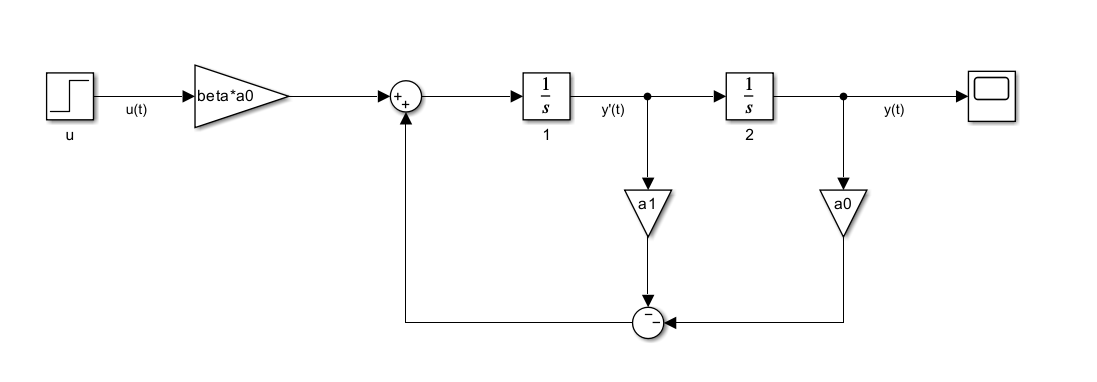
\includegraphics[width=\textwidth]{images/scheme1.png}
    \caption{Схема моделирования задания 1}
    \label{fig:1}
\end{figure}
На выходе первого интегратора получаем $\dot{y}$, поэтому его начальное значение равно $\dot{y}(0) = 0$. На выходе второго интегратора получаем $y$, его начальное значение равно $y(0)$.
\newline

\newpage
\subsection{Результаты моделирования}
\begin{figure}[H]
    \centering
    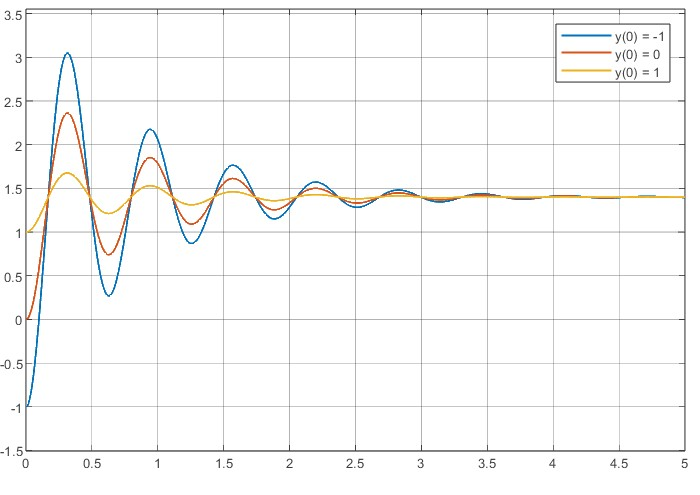
\includegraphics[width=0.8\textwidth]{images/exp2_u1.jpg}
    \caption{Эксперимент 2: $\lambda_{1,2} = -1.2 \pm 10j, u(t) = 1$}
    \label{fig:2}
\end{figure}
\begin{figure}[H]
    \centering
    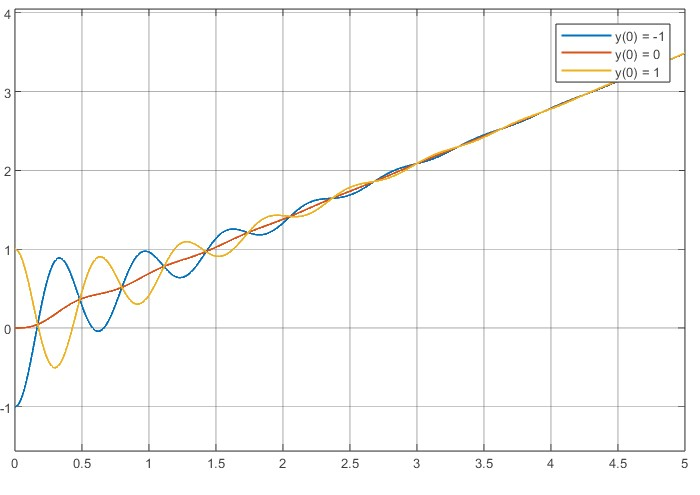
\includegraphics[width=0.8\textwidth]{images/exp2_u2.jpg}
    \caption{Эксперимент 2: $\lambda_{1,2} = -1.2 \pm 10j, u(t) = 0.5t$}
    \label{fig:2}
\end{figure}
\begin{figure}[H]
    \centering
    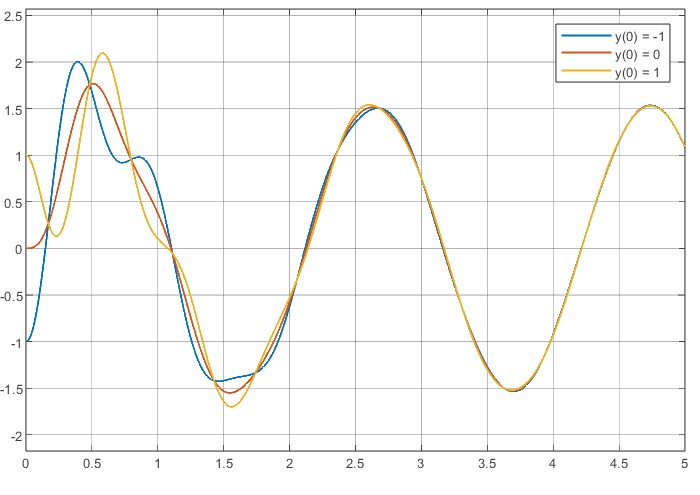
\includegraphics[width=0.8\textwidth]{images/exp2_u3.jpg}
    \caption{Эксперимент 2: $\lambda_{1,2} = -1.2 \pm 10j, u(t) = \sin{(3t)}$}
    \label{fig:2}
\end{figure}
\begin{figure}[H]
    \centering
    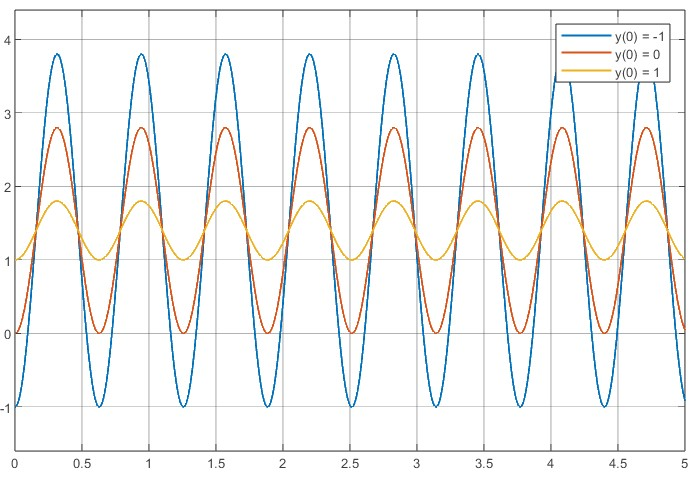
\includegraphics[width=0.8\textwidth]{images/exp3_u1.jpg}
    \caption{Эксперимент 3: $\lambda_{1,2} = \pm 10j, u(t) = 1$}
    \label{fig:2}
\end{figure}
\begin{figure}[H]
    \centering
    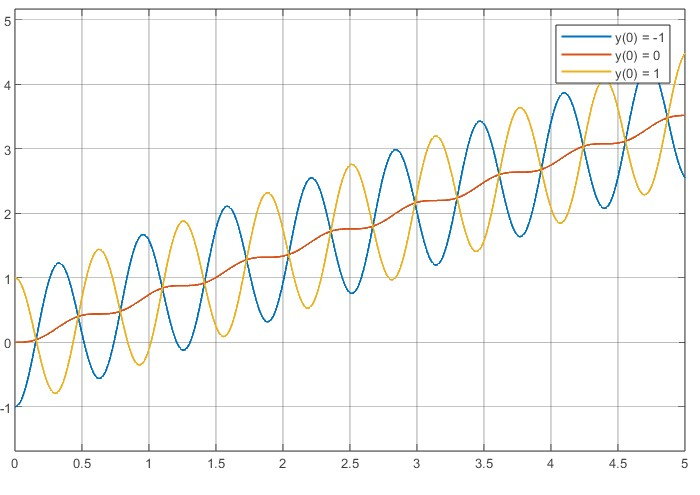
\includegraphics[width=0.8\textwidth]{images/exp3_u2.jpg}
    \caption{Эксперимент 3: $\lambda_{1,2} = \pm 10j, u(t) = 0.5t$}
    \label{fig:2}
\end{figure}
\begin{figure}[H]
    \centering
    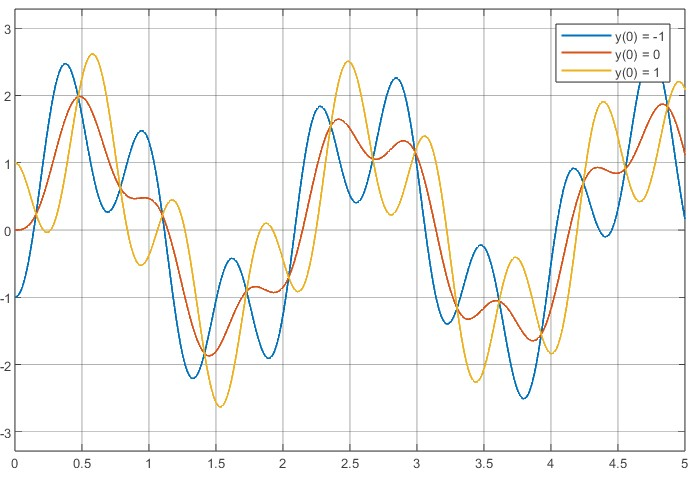
\includegraphics[width=0.8\textwidth]{images/exp3_u3.jpg}
    \caption{Эксперимент 3: $\lambda_{1,2} = \pm 10j, u(t) = \sin{(3t)}$}
    \label{fig:2}
\end{figure}
\begin{figure}[H]
    \centering
    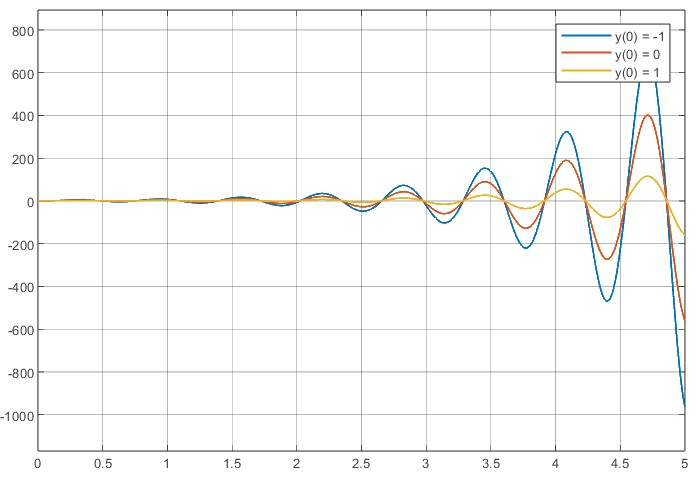
\includegraphics[width=0.8\textwidth]{images/exp4_u1.jpg}
    \caption{Эксперимент 4: $\lambda_{1,2} = 1.2 \pm 10j, u(t) = 1$}
    \label{fig:2}
\end{figure}
\begin{figure}[H]
    \centering
    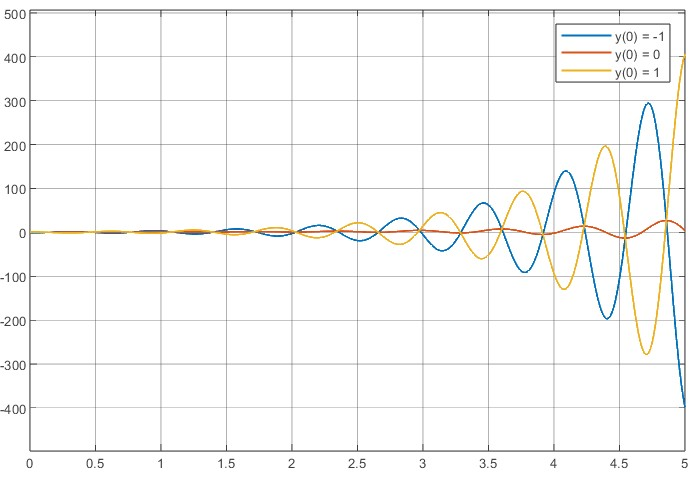
\includegraphics[width=0.8\textwidth]{images/exp4_u2.jpg}
    \caption{Эксперимент 4: $\lambda_{1,2} = 1.2 \pm 10j, u(t) = 0.5t$}
    \label{fig:2}
\end{figure}
\begin{figure}[H]
    \centering
    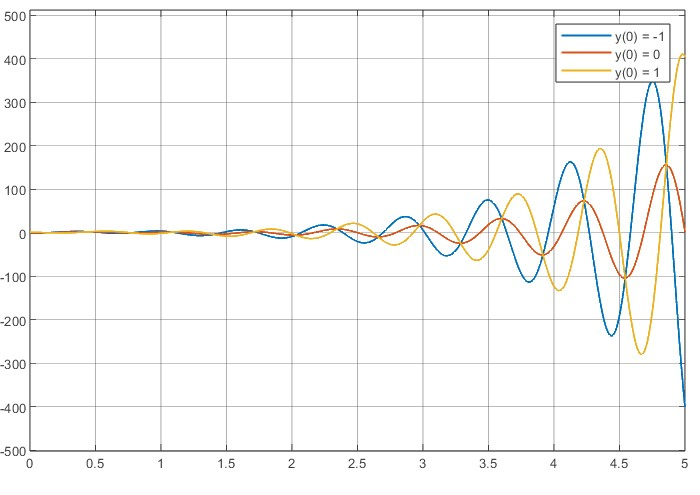
\includegraphics[width=0.8\textwidth]{images/exp4_u3.jpg}
    \caption{Эксперимент 4: $\lambda_{1,2} = 1.2 \pm 10j, u(t) = \sin{(3t)}$}
    \label{fig:2}
\end{figure}
\newpage
\subsection{Выводы по заданию 1}
Кривая при $y(0) = 0$ на каждом рисунке является вынужденной составляющей движения $y_{\text{в}}(t)$, а кривые при $y(0) = \pm 1$ отличаются от нее на $\pm$ свободную составляющую, поэтому расположены симметрично относительно нее. Это подтверждает, что движение системы равно сумме свободной и вынужденной составляющих. Графики соответствуют полученным аналитическим выражениям, например, в эксперименте 3 при $u = 1$ кривая с $y(0) = 0$ колеблется в пределах от $0$ до $2.8$, как и $y_{\text{в}}(t) = 1.4 - 1.4\cos{(10t)}$.

В эксперименте 2 система асимптотически устойчива. Свободная составляющая затухает за время порядка $4/1.2 \approx 3.3$ с (степень устойчивости $1.2$), после чего все три кривые сливаются: установившееся движение не зависит от начальных условий и определяется только входным воздействием:
\begin{align*}
    u = 1&: \quad y_{\text{у}}(t) = 1.4 \\
    u = 0.5t&: \quad y_{\text{у}}(t) = 0.7t - 0.0166 \\
    u = \sin{(3t)}&: \quad y_{\text{у}}(t) = 1.527\sin{(3t)} - 0.119\cos{(3t)} \approx 1.532\sin{(3t - 4.45^\circ)}
\end{align*}

В эксперименте 3 система находится на границе устойчивости. Собственные моды $\cos{(10t)}$ и $\sin{(10t)}$ не затухают, поэтому кривые не сходятся: к частному решению добавляются незатухающие колебания с частотой $10$ рад/с. Они присутствуют и при нулевых начальных условиях, так как вынужденная составляющая содержит собственные моды системы. Движение остается ограниченным, поскольку частота входного сигнала $3$ рад/с не совпадает с собственной частотой $10$ рад/с; при $u = \sin{(10t)}$ возник бы резонанс и амплитуда колебаний росла бы пропорционально $t$.

В эксперименте 4 система неустойчива. Все кривые, в том числе при нулевых начальных условиях, неограниченно растут: вынужденная составляющая неустойчивой системы также содержит растущие моды. Начальные условия влияют только на амплитуду и фазу расходящихся колебаний. При $u = 1$ медленнее всех расходится кривая с $y(0) = 1$, так как она начинается ближе всех к положению равновесия $y = 1.4$.
\newpage


\section{Задание №2}

\subsection{Исходные данные}
Рассматриваем системы третьего порядка с передаточной функцией
\[
    W(s) = \frac{|\lambda_1 \lambda_2 \lambda_3|}{(s - \lambda_1)(s - \lambda_2)(s - \lambda_3)}
\]
Для варианта 13  $a = 9$, $b = 19$, $c = 33$. Так как номер варианта нечетный, принимаем $\delta_{\text{п}} = 2\%$.
\begin{table}[H]
\centering
\renewcommand{\arraystretch}{2.3}
\caption{Полюсы и передаточные функции систем для задания 2}
\label{tab:3}
\begin{tabular}{|c|c|c|c|c|}
    \hline
    \textnumero & $\lambda_1$ & $\lambda_2$ & $\lambda_3$ & $W(s)$ \\ \hline
    1 & $-9$ & $-9$ & $-9$ & $\dfrac{729}{s^3 + 27s^2 + 243s + 729}$ \\ \hline
    2 & $-9$ & $-19$ & $-19$ & $\dfrac{3249}{s^3 + 47s^2 + 703s + 3249}$ \\ \hline
    3 & $-9$ & $-33$ & $-33$ & $\dfrac{9801}{s^3 + 75s^2 + 1683s + 9801}$ \\ \hline
    4 & $-9$ & $-19 + 33i$ & $-19 - 33i$ & $\dfrac{13050}{s^3 + 47s^2 + 1792s + 13050}$ \\ \hline
    5 & $-33$ & $-9 + 9i$ & $-9 - 9i$ & $\dfrac{5346}{s^3 + 51s^2 + 756s + 5346}$ \\ \hline
    6 & $-33$ & $-9 + 33i$ & $-9 - 33i$ & $\dfrac{38610}{s^3 + 51s^2 + 1764s + 38610}$ \\ \hline
\end{tabular}
\end{table}
Составим схему системы в Simulink в форме вход-выход:
\begin{figure}[H]
    \centering
    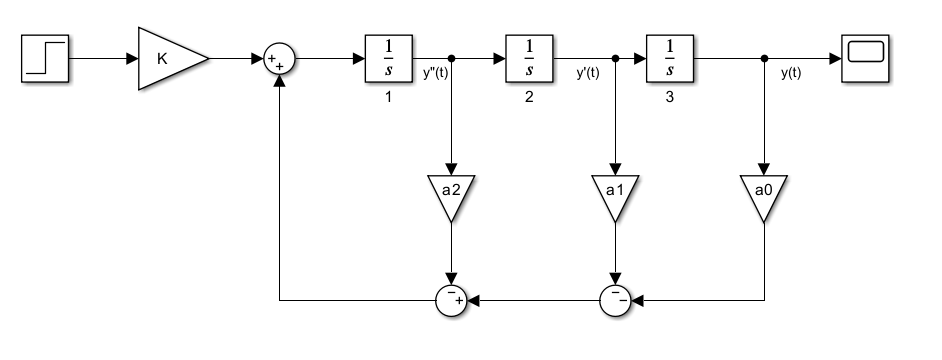
\includegraphics[width=\textwidth]{images/scheme2.png}
    \caption{Схема моделирования задания 2}
    \label{fig:1}
\end{figure}
\subsection{Корневые показатели качества и оценки динамических показателей}
Степень устойчивости и степень колебательности:
\[
    \eta = \min_i |\mathrm{Re}\,\lambda_i|, \qquad \mu = \max_i \left|\frac{\mathrm{Im}\,\lambda_i}{\mathrm{Re}\,\lambda_i}\right|
\]
Во всех экспериментах ближайший к мнимой оси полюс имеет вещественную часть $-9$, поэтому $\eta = 9$. В экспериментах 1--3 все полюсы вещественные, $\mu = 0$. Для остальных:
\[
    \mu_4 = \frac{33}{19} \approx 1.737, \qquad \mu_5 = \frac{9}{9} = 1, \qquad \mu_6 = \frac{33}{9} \approx 3.667
\]
Оценка времени переходного процесса:
\[
    t^*_{\text{п}} = \frac{1}{\eta}\ln{\frac{1}{\delta_{\text{п}}}} = \frac{\ln{50}}{9} \approx 0.435 \ \text{с}
\]
Она одинакова для всех экспериментов, так как $\eta$ одинакова.
\newline
Оценка перерегулирования $\sigma^* = e^{-\frac{\pi}{\mu}} \cdot 100\%$ (при $\mu = 0$ принимаем $\sigma^* = 0$):
\[
    \sigma^*_4 = e^{-\frac{19\pi}{33}} \cdot 100\% \approx 16.39\%, \qquad
    \sigma^*_5 = e^{-\pi} \cdot 100\% \approx 4.32\%, \qquad
    \sigma^*_6 = e^{-\frac{9\pi}{33}} \cdot 100\% \approx 42.45\%
\]

\subsection{Переходные характеристики}
Для переходных характеристикик $h(t)$  время переходного процесса $t_{\text{п}}$ определено как момент, после которого выполняется $|h(t) - 1| \le \delta_{\text{п}} = 0.02$, перерегулирование как
\[
    \sigma = \frac{h_{\max} - 1}{1} \cdot 100\% \ \ \textit{при} \ \ h_{\max} > 1, \qquad \sigma = 0 \ \ \textit{иначе}
\]
\begin{figure}[H]
    \centering
    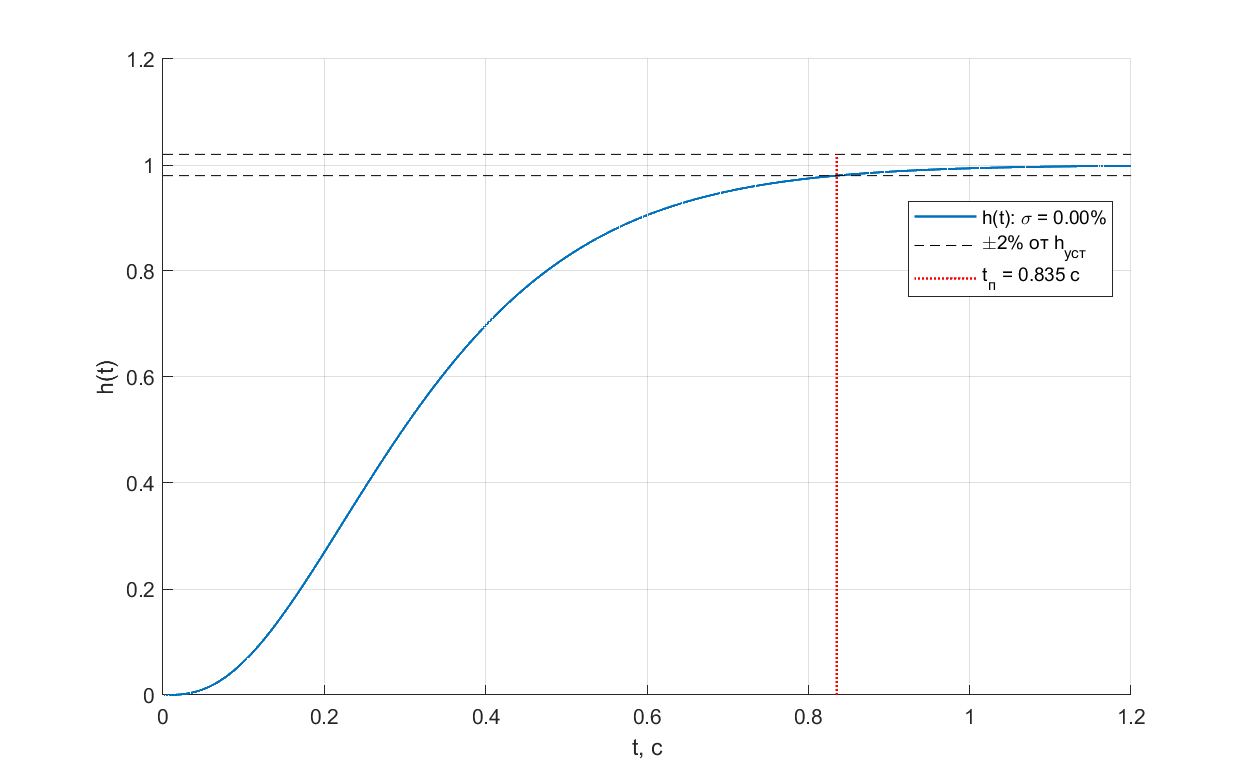
\includegraphics[width=0.8\textwidth]{images/task2_exp1.png}
    \caption{Переходная характеристика системы для 1 набора}
    \label{fig:2}
\end{figure}
\begin{figure}[H]
    \centering
    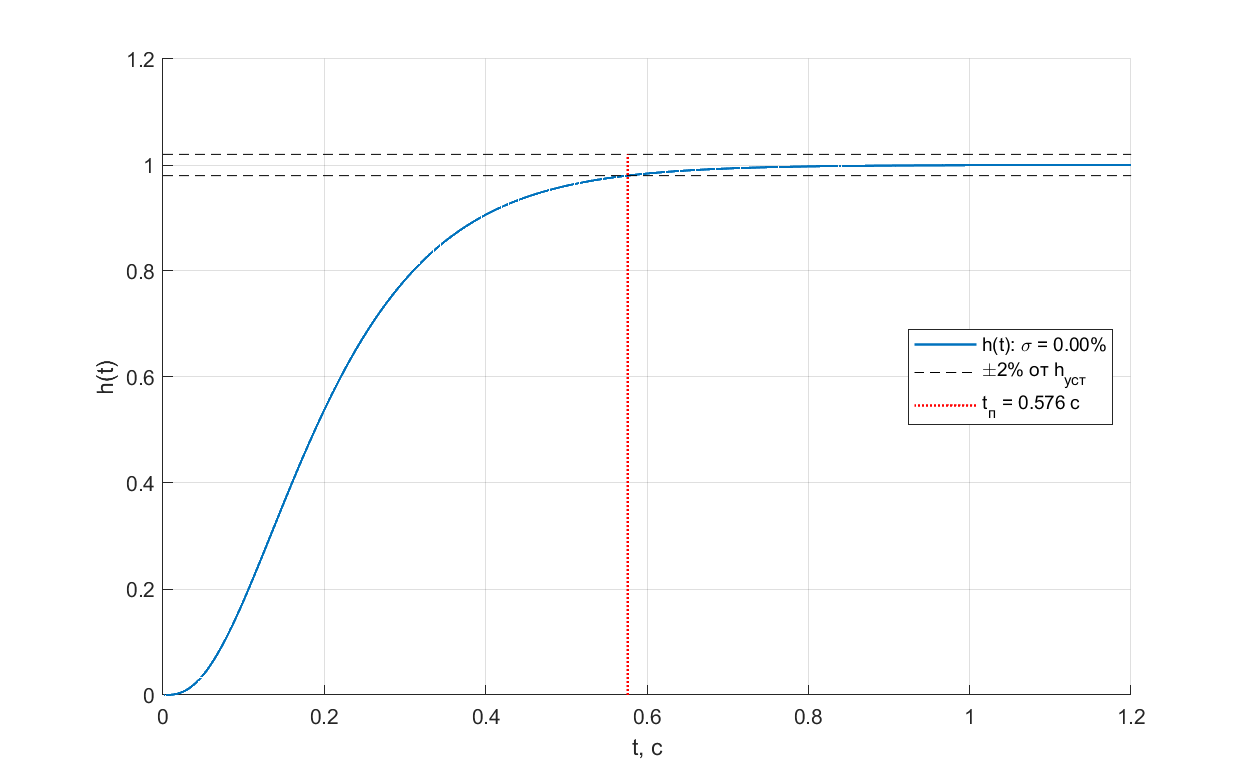
\includegraphics[width=0.8\textwidth]{images/task2_exp2.png}
    \caption{Переходная характеристика системы для 2 набора}
    \label{fig:2}
\end{figure}
\begin{figure}[H]
    \centering
    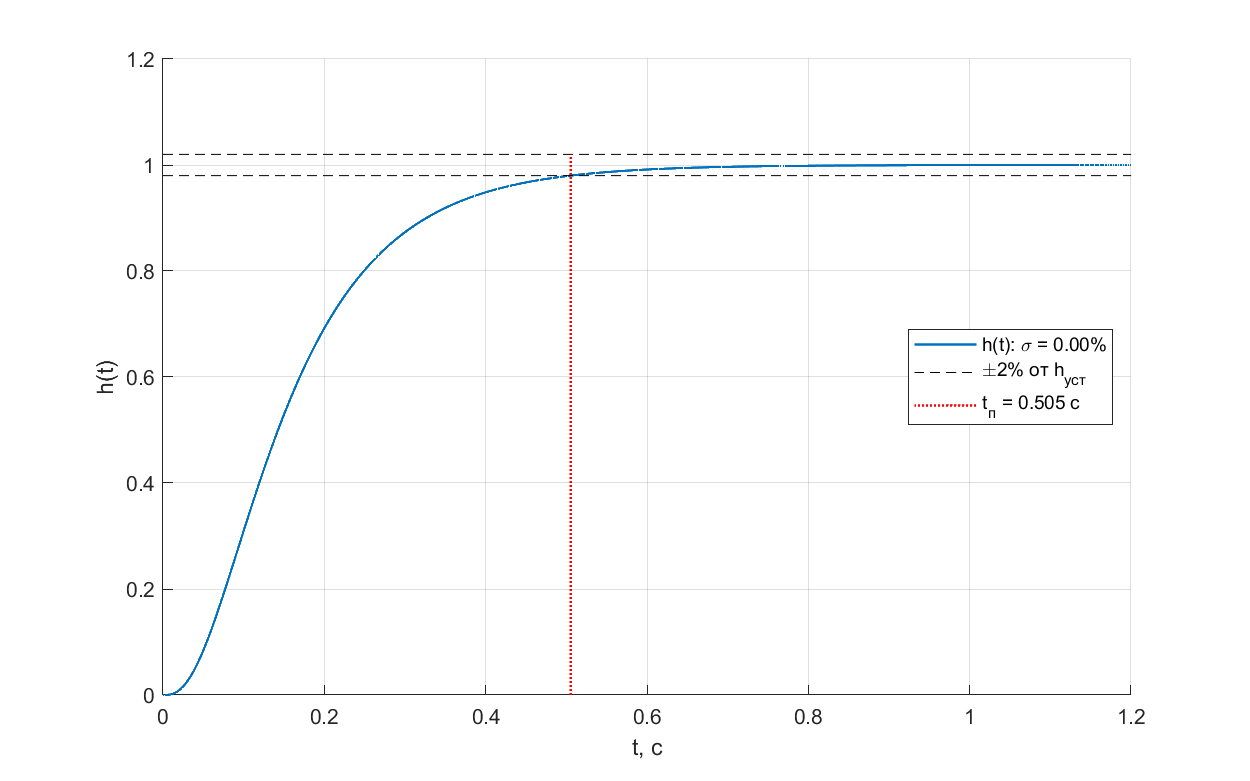
\includegraphics[width=0.8\textwidth]{images/task2_exp3.png}
    \caption{Переходная характеристика системы для 3 набора}
    \label{fig:2}
\end{figure}
\begin{figure}[H]
    \centering
    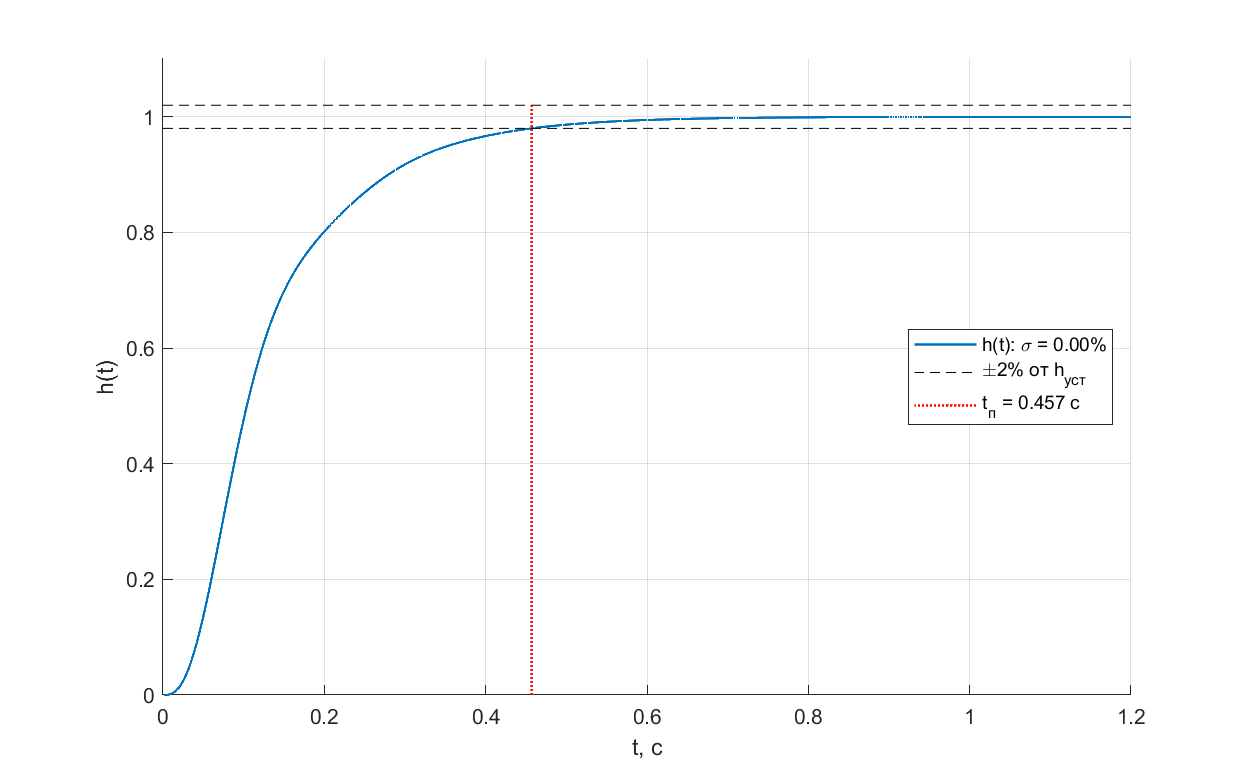
\includegraphics[width=0.8\textwidth]{images/task2_exp4.png}
    \caption{Переходная характеристика системы для 4 набора}
    \label{fig:2}
\end{figure}
\begin{figure}[H]
    \centering
    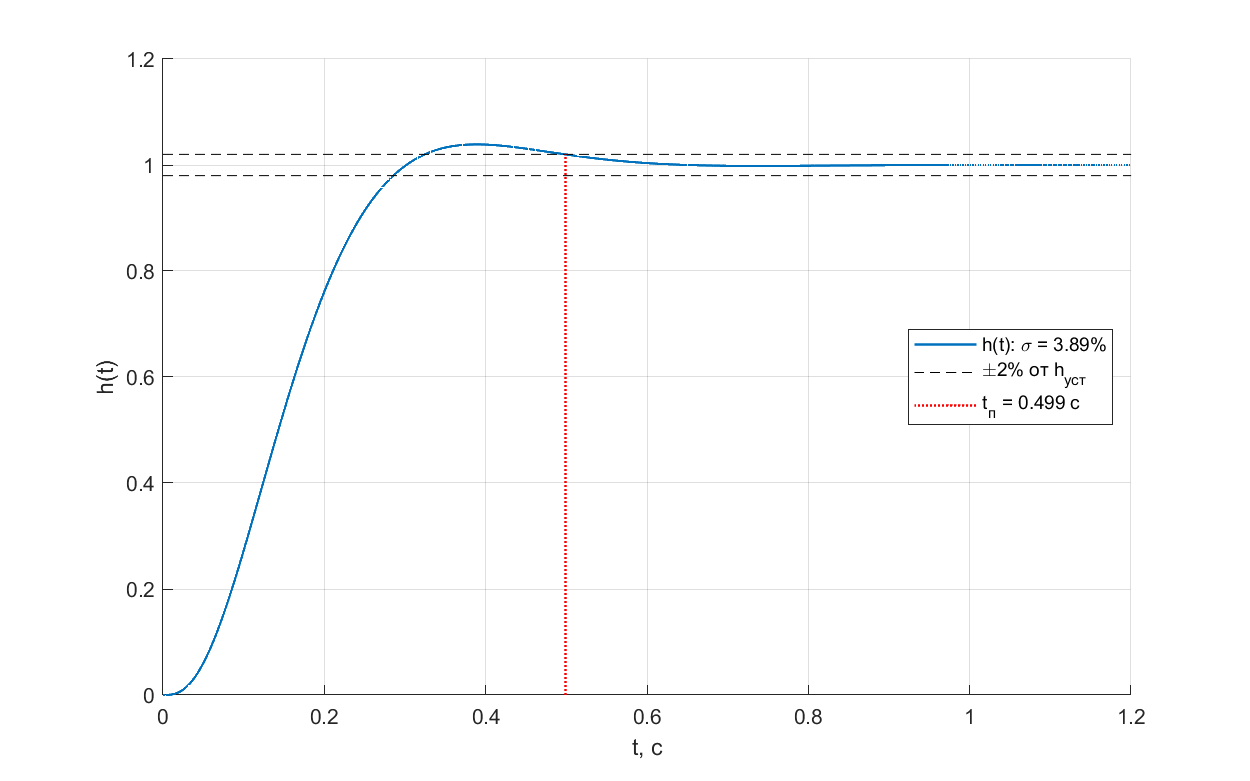
\includegraphics[width=0.8\textwidth]{images/task2_exp5.png}
    \caption{Переходная характеристика системы для 5 набора}
    \label{fig:2}
\end{figure}
\begin{figure}[H]
    \centering
    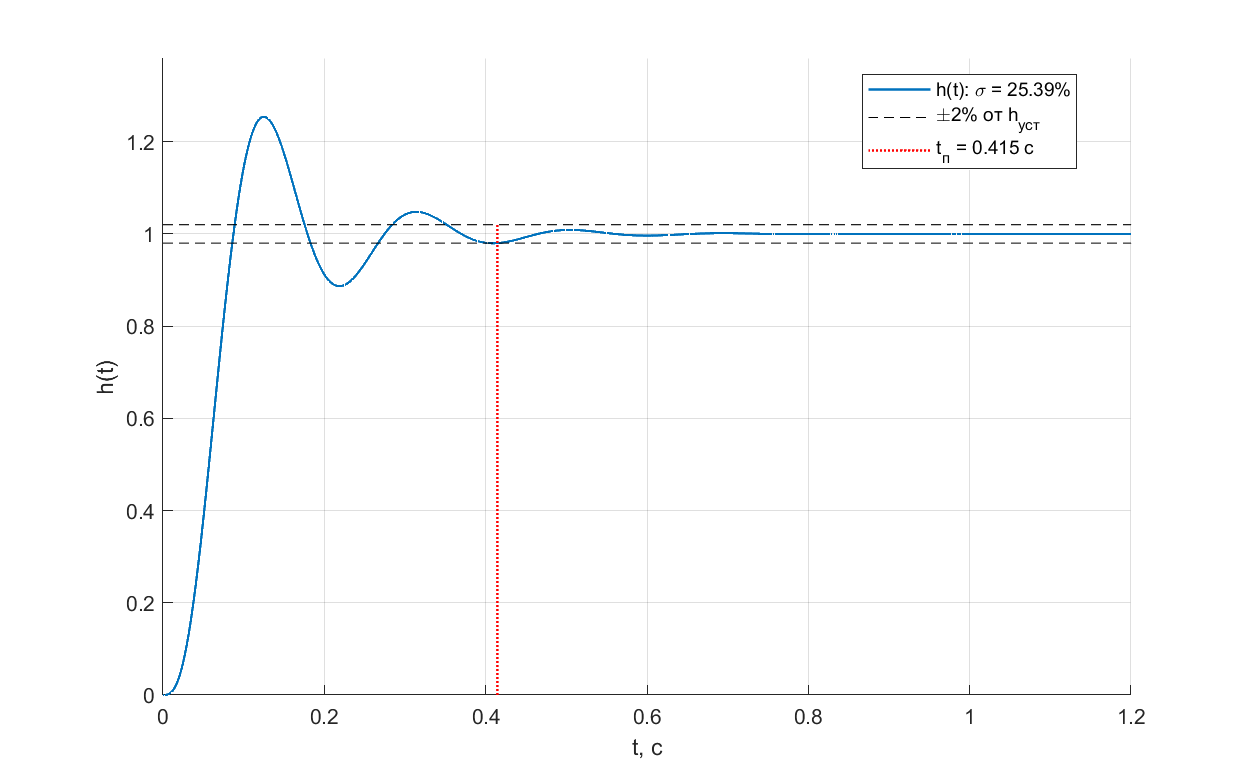
\includegraphics[width=0.8\textwidth]{images/task2_exp6.png}
    \caption{Переходная характеристика системы для 6 набора}
    \label{fig:2}
\end{figure}


\subsection{Результаты расчетов}
\begin{table}[H]
\centering
\caption{Результаты вычислений для задания 2}
\label{tab:4}
\setlength{\tabcolsep}{3pt}
\begin{tabular}{|c|c|c|c|c|c|c|c|c|c|}
    \hline
    \multirow{2}{*}{\textnumero} & \multicolumn{3}{c|}{Корни} & \multicolumn{2}{c|}{\makecell{Корневые показатели \\ качества}} & \multicolumn{2}{c|}{\makecell{Оценки динамических \\ показателей качества}} & \multicolumn{2}{c|}{\makecell{Динамические \\ показатели качества}} \\ \cline{2-10}
    & $\lambda_1$ & $\lambda_2$ & $\lambda_3$ & $\eta$ & $\mu$ & $t^*_{\text{п}}$, с & $\sigma^*$, \% & $t_{\text{п}}$, с & $\sigma$, \% \\ \hline
    1 & $-9$ & $-9$ & $-9$ & $9$ & $0$ & $0.435$ & $0$ & $0.835$ & $0$ \\ \hline
    2 & $-9$ & $-19$ & $-19$ & $9$ & $0$ & $0.435$ & $0$ & $0.576$ & $0$ \\ \hline
    3 & $-9$ & $-33$ & $-33$ & $9$ & $0$ & $0.435$ & $0$ & $0.505$ & $0$ \\ \hline
    4 & $-9$ & $-19 + 33i$ & $-19 - 33i$ & $9$ & $1.737$ & $0.435$ & $16.39$ & $0.457$ & $0$ \\ \hline
    5 & $-33$ & $-9 + 9i$ & $-9 - 9i$ & $9$ & $1$ & $0.435$ & $4.32$ & $0.499$ & $3.89$ \\ \hline
    6 & $-33$ & $-9 + 33i$ & $-9 - 33i$ & $9$ & $3.667$ & $0.435$ & $42.45$ & $0.415$ & $25.39$ \\ \hline
\end{tabular}
\end{table}

\newpage
\subsection{Выводы по заданию 2}
Во всех шести экспериментах степень устойчивости одинакова, поэтому оценка $t^*_{\text{п}} \approx 0.435$ с одна и та же, тогда как фактическое время переходного процесса меняется от $0.415$ до $0.835$ с. Оценка достаточно точна, когда доминантный полюс отделен от остальных (эксперименты 3--6, отклонение не больше $0.07$ с), и заметно занижает $t_{\text{п}}$ при кратных и близко расположенных полюсах: в эксперименте 1 (тройной полюс $-9$) время переходного процесса почти вдвое больше оценки, в эксперименте 2 больше на $0.14$ с.

В экспериментах 1--3 все полюсы вещественные и нули отсутствуют, поэтому переходные процессы апериодические и $\sigma = \sigma^* = 0$.

В эксперименте 4 оценка дает $\sigma^* \approx 16.39\%$, однако перерегулирования нет. Степень колебательности здесь определяется быстрой парой $-19 \pm 33i$, а доминантным является вещественный полюс $-9$, поэтому колебательная составляющая затухает раньше, чем процесс подходит к установившемуся значению. Оценка по степени колебательности применима, только если $\mu$ определяется доминантными корнями.

В эксперименте 5 степень колебательности определяется доминантной парой $-9 \pm 9i$, и оценка $\sigma^* = 4.32\%$ близка к фактическому $\sigma = 3.89\%$.

В эксперименте 6 оценка $\sigma^* = 42.45\%$ оказалась верхней: фактическое перерегулирование $25.39\%$. Третий полюс $-33$ по модулю сравним с доминантной парой ($|-9 \pm 33i| \approx 34.2$) и сглаживает колебания.
\newpage


\section{Выводы}
В лабораторной работе исследовано вынужденное движение линейной системы второго порядка для трех наборов корней характеристического уравнения, соответствующих асимптотически устойчивой системе, системе на границе устойчивости и неустойчивой системе, при постоянном, линейно нарастающем и гармоническом входных воздействиях. Вынужденные составляющие движения найдены аналитически, а моделирование при различных начальных условиях подтвердило, что движение системы равно сумме свободной и вынужденной составляющих. Установившееся движение существует только у асимптотически устойчивой системы и определяется лишь входным воздействием; у системы на границе устойчивости сохраняются незатухающие собственные колебания, а у неустойчивой системы расходится и вынужденная составляющая.

Для шести систем третьего порядка определены корневые показатели качества (степень устойчивости и степень колебательности) и динамические показатели (время переходного процесса и перерегулирование). Сравнение показало, что корневые оценки дают лишь ориентировочный результат: оценка времени переходного процесса точна при отделенном доминантном полюсе и занижена при кратных полюсах, а оценка перерегулирования применима, только когда степень колебательности определяется доминантной парой корней, и в остальных случаях может значительно отличаться от фактического значения.
\end{document}

